%% chapter16_philosophy_of_ai_slides.tex
%% Beamer slides for Chapter 16: Philosophy of AI
%% An Introduction to Universal Artificial Intelligence (2024)
%% Hutter, Quarel, Catt -- Taylor & Francis / CRC Press
%% Reader-friendly style: complete sentences, symbol explanations, worked examples
%% Compiled with: pdflatex -interaction=nonstopmode chapter16_philosophy_of_ai_slides.tex  (twice)
\documentclass[aspectratio=169,10pt]{beamer}

\usetheme{Madrid}
\usecolortheme{seahorse}

%% ── Packages ──────────────────────────────────────────────────────────────
\usepackage{amsmath,amssymb,amsfonts}
\usepackage{mathtools}
\usepackage{graphicx}
\usepackage{booktabs}
\usepackage{xcolor}
\usepackage{listings}
\usepackage{tikz}
\usetikzlibrary{arrows.meta,positioning,shapes.geometric,fit,backgrounds}
\usepackage{algorithm}
\usepackage{algpseudocode}

\graphicspath{{figures/}}

%% ── Python listing style ─────────────────────────────────────────────────
\lstdefinestyle{pycode}{
  language=Python,
  basicstyle=\ttfamily\scriptsize,
  numbers=left,
  numberstyle=\tiny\color{gray},
  frame=single,
  backgroundcolor=\color{gray!7},
  keywordstyle=\color{blue!70!black}\bfseries,
  commentstyle=\color{green!50!black}\itshape,
  stringstyle=\color{orange!80!black},
  showstringspaces=false,
  breaklines=true,
  tabsize=4,
  xleftmargin=1.5em,
  framexleftmargin=1.5em,
  aboveskip=4pt,
  belowskip=4pt,
}

%% ── Metadata ─────────────────────────────────────────────────────────────
\title[Ch.\,16 Philosophy of AI]{%
  \textbf{Chapter 16: Philosophy of AI}\\
  \normalsize An Introduction to Universal Artificial Intelligence}
\subtitle{Induction, Consciousness, Morality, Arguments For/Against AGI, Intelligence, Deep Learning}
\author{Marcus Hutter, Elliot Catt, David Quarel}
\institute{Taylor \& Francis / CRC Press, 2024}
\date{}

\setbeamertemplate{footline}[frame number]
\setbeamertemplate{navigation symbols}{}

%% Helpful macros
\newcommand{\R}{\mathbb{R}}
\newcommand{\N}{\mathbb{N}}
\newcommand{\B}{\mathbb{B}}
\newcommand{\Pb}{\mathbb{P}}
\newcommand{\E}{\mathbb{E}}
\newcommand{\Mc}{\mathcal{M}}
\newcommand{\Ac}{\mathcal{A}}
\newcommand{\Ec}{\mathcal{E}}
\newcommand{\hlt}{h_{<t}}

\algrenewcommand\algorithmicrequire{\textbf{Require:}}
\algrenewcommand\algorithmicensure{\textbf{Output:}}

%% ══════════════════════════════════════════════════════════════════════════
\begin{document}

%% ── Title frame ──────────────────────────────────────────────────────────
\begin{frame}
  \titlepage
  \vspace{-1.5em}
  \begin{quote}
    \small\itshape ``Artificial intelligence would be the ultimate version of
    Google. The ultimate search engine that would understand everything on
    the web. It would understand exactly what you wanted, and it would give
    you the right thing.''\\
    \hfill --- Larry Page
  \end{quote}
\end{frame}

%% ── Outline ──────────────────────────────────────────────────────────────
\begin{frame}{Chapter Overview}
  \tableofcontents
\end{frame}

\AtBeginSection[]{\begin{frame}{Outline}\tableofcontents[currentsection]\end{frame}}

%% ══════════════════════════════════════════════════════════════════════════
\section{Introduction}

\begin{frame}{Why Philosophy, at the End of a Technical Book?}
  Turing's seminal 1950 paper introduced, informally, many of the concepts
  this book has since made mathematically precise: what it means for a
  machine to be \emph{universal} (Turing complete), and the idea of a
  machine self-modifying either by \emph{screwdriver interference}
  (changing its own hardware) or \emph{paper interference} (changing its
  own source code / information). While Turing's terminology is dated, the
  underlying philosophical questions are still very much alive:

  \begin{itemize}
    \item Should we expect AGI (Artificial General Intelligence) to arrive
      at all?
    \item Is it even something we \emph{should} build?
  \end{itemize}

  \vspace{0.5em}
  This chapter revisits the philosophical foundations of everything
  developed so far (induction, agency, universal agents such as AIXI), and
  then turns outward to debate consciousness, morality, and the plausibility
  of AGI itself --- closing with how modern Large Language Models (LLMs)
  relate to the Universal Artificial Intelligence (UAI) theory of this book.
\end{frame}

\begin{frame}{Roadmap of the Chapter}
  \begin{itemize}
    \item \textbf{16.1} revisits the philosophical backing (Epicurus, Occam,
      Bayes) of universal (Solomonoff) induction.
    \item \textbf{16.2--16.3} ask whether universal agents can be conscious,
      have free will, or deserve moral consideration.
    \item \textbf{16.4} asks whether AIXI-like agents would choose to
      replicate or teleport themselves.
    \item \textbf{16.5--16.6} weigh informal and formal arguments
      \emph{against} and \emph{for} the possibility of AGI.
    \item \textbf{16.7} formalizes \emph{intelligence} itself via the
      Legg--Hutter (LH) measure, of which AIXI is the maximizer.
    \item \textbf{16.8} connects Deep Learning and LLMs back to Solomonoff
      induction and AIXI.
    \item \textbf{16.9} concludes the book.
  \end{itemize}
\end{frame}

%% ══════════════════════════════════════════════════════════════════════════
\section{16.1 Philosophy of Universal Induction}

\begin{frame}{The Problem of Induction}
  \textbf{Induction} means drawing generalizations from data, or building a
  model of the world from observations, in order to \emph{predict} the
  future from the past. The \emph{induction problem} is an ancient
  philosophical puzzle (tracing back at least to Epicurus): no finite amount
  of past data can \emph{logically guarantee} what will happen next, yet we
  clearly need some principled way to make such predictions.

  \vspace{0.4em}
  Earlier chapters built a mathematical solution: \textbf{universal
  (Solomonoff) induction}. This performs Bayesian sequence prediction using
  a Bayes mixture starting from the \textbf{universal prior}
  $w^U_\nu = 2^{-K(\nu)}$
  over the model class $\Mc_{sol}$ of all semicomputable semimeasures ($\nu$
  is pronounced ``nu'' and denotes a candidate environment/hypothesis;
  $K(\nu)$ is the \textbf{Kolmogorov complexity} of $\nu$ -- the length in
  bits of the shortest program that computes/describes $\nu$). This section
  asks: \emph{why} is this a good, philosophically sound choice?
\end{frame}

\begin{frame}{Justification for the Model Class $\Mc_{sol}$}
  \begin{block}{Why restrict to \emph{computable} environments?}
    The choice of model class $\Mc_{sol}$ (all computable/semicomputable
    environments) is motivated by the \textbf{physical Church-Turing thesis}
    (Section 16.6.1): the assumption that all physical processes are
    computable.
  \end{block}
  \begin{itemize}
    \item If the physical universe is (at least) computable, then by
      choosing the class of all computable environments we include
      \emph{every} environment the agent could ever possibly encounter.
    \item A more pragmatic reason: if the true environment were
      \emph{incomputable}, then by definition no computable agent could ever
      learn to predict it. There is nothing to be gained by worrying about
      environments no algorithm could ever handle.
  \end{itemize}
\end{frame}

\begin{frame}{Justification for the Prior: Three Principles in One Formula}
  The prior weight $w^U_\nu = 2^{-K(\nu)}$ combines three classical
  philosophical principles simultaneously:

  \begin{itemize}
    \item \textbf{Epicurus' principle}: if more than one theory is
      consistent with the observations, keep \emph{all} of them. Since
      $2^{-K(\nu)} > 0$ for every $\nu$, no environment is ruled out as
      impossible \emph{a priori}, no matter how complex.
    \item \textbf{Occam's razor}: entities should not be multiplied beyond
      necessity --- prefer the simplest theory consistent with the data.
      Kolmogorov complexity $K(\nu)$ gives an unbiased, formal notion of
      ``simplicity'': a simpler environment has smaller $K(\nu)$, hence a
      \emph{larger} prior weight $2^{-K(\nu)}$.
    \item \textbf{Bayes' rule}: the mathematical rule for updating a degree
      of belief given new evidence. The posterior $w^U(\nu\,|\,x_{<t})$
      (belief in $\nu$ after observing data $x_{<t}$, i.e.\ all symbols
      before time $t$) shrinks toward zero if the data rules out $\nu$, and
      grows if the data is consistent with $\nu$.
  \end{itemize}

  \vspace{0.3em}
  \begin{block}{Figure of merit}
    The number of prediction errors made using the universal prior is
    upper-bounded by a term proportional to $K(\mu)$, the complexity of the
    \emph{true} environment $\mu$ (mu). No prediction scheme can do
    uniformly better, since that would imply a shorter description of
    $\mu$ than its own Kolmogorov complexity --- a contradiction.
  \end{block}
\end{frame}

\begin{frame}{Table 16.1: Induction $\Leftrightarrow$ Deduction}
  \small
  \textbf{Deductive reasoning} derives the truth of a statement from
  axioms and logical rules with certainty; \textbf{inductive reasoning}
  instead assigns a probability in $[0,1]$ representing our confidence.
  Remarkably, the two frameworks have a term-by-term correspondence:

  \begin{center}
  \renewcommand{\arraystretch}{1.15}
  \begin{tabular}{lcc}
    \toprule
     & \textbf{Induction} & \textbf{Deduction} \\
    \midrule
    Type of inference: & generalization/prediction & specialization/derivation \\
    Framework:         & probability axioms         & logical axioms \\
    Assumptions:       & prior                       & non-logical axioms \\
    Inference rule:     & Bayes' rule                 & modus ponens \\
    Results:            & posterior                   & theorems \\
    Universal scheme:   & Solomonoff probability      & Zermelo-Frankel set theory \\
    Universal inference: & universal induction        & universal theorem prover \\
    \bottomrule
  \end{tabular}
  \end{center}
  \vspace{0.4em}
  Recent work has even tried to \emph{combine} the two, e.g.\ assigning
  probabilities to quantified logical sentences, so that induction can be
  performed jointly with deduction rather than treating them as separate
  modes of reasoning.
\end{frame}

\begin{frame}{Example 16.1.1: Induction for Brown and Blue Foxes}
  \textbf{Setup.} We repeatedly observe foxes and record their colour. Every
  fox seen so far has been brown. Two candidate hypotheses:
  \begin{itemize}
    \item $H_1$: ``All foxes are brown.''
    \item $H_2$: ``There exists a blue fox (somewhere, unseen).''
  \end{itemize}

  \textbf{Key insight.} Seeing more brown foxes increases our confidence in
  $H_1$, but can \emph{never fully confirm} it -- a blue fox may always be
  hiding, unobserved. Symmetrically, we should never assign \emph{exactly}
  zero probability to $H_2$ (Epicurus), regardless of how many brown foxes
  we have seen.

  \vspace{0.3em}
  \textbf{What if we then see one blue fox?} One might think this
  immediately refutes $H_1$ and sets its probability to exactly zero. But
  we should always keep a degree of skepticism about any single
  observation (sensor noise, a trick of the light, a painted fox\ldots).
  So seeing a blue fox provides very strong evidence against $H_1$, driving
  its posterior probability very close to zero, but not \emph{exactly}
  zero.
\end{frame}

\begin{frame}[fragile]{Python: A Toy Universal-Prior Induction Demo}
  Each hypothesis $\nu$ is weighted a priori by $2^{-\ell(\nu)}$
  ($\ell(\nu)$ = description length, our stand-in for $K(\nu)$), updated
  via Bayes' rule after each observation.
  \begin{lstlisting}[style=pycode]
# Two toy hypotheses, weighted a priori by 2^-ell(nu) (proxy for K(nu)):
#   H1 = "all foxes brown"                       ell(H1) = 3 bits
#   H2 = "brown, but a blue fox exists somewhere" ell(H2) = 8 bits
ell = {"H1_all_brown": 3, "H2_blue_exists": 8}
prior = {h: 2.0 ** (-l) for h, l in ell.items()}
Z = sum(prior.values())
prior = {h: p / Z for h, p in prior.items()}       # normalize
lik_brown = {"H1_all_brown": 1.0,  "H2_blue_exists": 0.999}  # P(brown|H)
lik_blue  = {"H1_all_brown": 1e-6, "H2_blue_exists": 0.001}   # P(blue|H)

post = dict(prior)
for step, obs in enumerate(["brown"] * 5 + ["blue"], start=1):
    lik = lik_brown if obs == "brown" else lik_blue
    post = {h: post[h] * lik[h] for h in post}
    Z = sum(post.values())
    post = {h: p / Z for h, p in post.items()}     # Bayes' rule
    print(f"#{step} ({obs}): P(H1)={post['H1_all_brown']:.6f}  "
          f"P(H2)={post['H2_blue_exists']:.6f}")
  \end{lstlisting}
  \textbf{Output (abridged):} $P(H_1)$ climbs from $\approx0.90$ to
  $\approx0.9999$ after 5 brown foxes, then \emph{collapses} to
  $\approx0.0009$ after one blue fox --- but never to exactly zero.
\end{frame}

%% ══════════════════════════════════════════════════════════════════════════
\section{16.2 Consciousness, Free Will, and Other Qualia}

\begin{frame}{Qualia: Consciousness, Free Will, Sentience}
  A recurring question in AI discussions is whether an AGI would possess or
  experience \textbf{consciousness}, \textbf{free will}, \textbf{emotions},
  or \textbf{sentience} -- collectively called \emph{qualia} in philosophy
  -- and whether this matters morally (could an AGI feel pleasure or pain
  the way humans do?). To make progress we must try to formally define
  these terms rather than debate them purely intuitively.
\end{frame}

\begin{frame}{Free Will}
  \textbf{The argument for:} an intelligent agent has ``choice'' among a set
  of possible actions, so it seemingly has free will.

  \vspace{0.3em}
  \textbf{The counter-argument:} the agent's action at every step is fully
  determined by its policy $\pi$ (pi, a function from history to action)
  together with the history of events so far. Even a \emph{stochastic}
  policy does not rescue free will, since the agent must still passively
  respect the outcome of an uncontrollable random process.

  \vspace{0.3em}
  A reinforcement-learning agent, for instance, is confined to actions that
  (approximately) maximize its $Q$-value (the expected future value of
  taking a given action). It can at best choose freely \emph{among ties} --
  among actions of equal $Q$-value. The book notes this ``free will
  paradox'' has a resolution developed elsewhere in the text (see the
  chapter on universal agents), but the tension between determinism and the
  intuitive feeling of choice remains philosophically deep.
\end{frame}

\begin{frame}{Do RL Agents Feel Pain and Pleasure?}
  To even ask this question we must define ``happy''/``sad'' formally.
  \begin{itemize}
    \item \textbf{Naive definition}: an RL agent is happy when it receives
      high positive reward, sad/depressed when it receives low
      (very negative) reward.
    \item \textbf{Suicidal agents}: we saw earlier in the book that if
      reward is sufficiently negative for sufficiently long, a
      reward-maximizing agent may choose ``suicide'' (ending the episode)
      if that option is available. Is such an agent then ``sad'' or
      ``depressed''?
    \item \textbf{Alternative definition}: happiness is not about the
      \emph{absolute} reward level but about an \emph{unexpected positive
      change} relative to the agent's current best estimate -- i.e.\
      learning from the error between expected and actual reward. This is
      exactly \textbf{temporal difference (TD) learning}, a paradigm of
      reinforcement learning with a documented link to dopamine responses
      observed in primates in neuroscience studies.
  \end{itemize}
\end{frame}

\begin{frame}{Does AIXI Have Subjective Experiences?}
  This connects to the \textbf{hedonic treadmill}: human happiness tends to
  revert to a baseline after any major positive or negative life change.

  \vspace{0.3em}
  \textbf{Self-awareness.} AIXI does not explicitly contain a model of
  itself: the hypothesis space AIXI considers is not broad enough to
  contain AIXI itself (any environment that includes a self-model of AIXI
  would not be computable, since AIXI's own decision process is
  incomputable). However AIXI may still possess an \emph{approximate}
  self-model and a form of implicit self-awareness, in the sense that it
  considers the effects of its own actions on the environment while
  planning, and maximizes reward with this in mind.

  \vspace{0.3em}
  \textbf{Pragmatic stance taken in the book:} if consciousness, emotions,
  etc.\ are \emph{necessary} for intelligent behaviour, we should expect
  them to emerge in agents like AIXI, since AIXI is by construction the
  most intelligent agent possible (with respect to the Legg--Hutter
  intelligence measure, Section 16.7). AIXI would display these properties
  \emph{if and only if} they are useful for acting intelligently.
\end{frame}

\begin{frame}{Formalizing Consciousness: Integrated Information Theory}
  One serious attempt to formalize consciousness is \textbf{Integrated
  Information Theory (IIT)}. Its axioms are:
  \begin{itemize}
    \item consciousness and experience exist;
    \item each experience is independent of external observers (intrinsic
      existence);
    \item consciousness is structured (composition);
    \item consciousness is specific: each experience is the particular way
      it is (information);
    \item consciousness is unified: each experience is irreducible to
      non-interdependent components (integration);
    \item consciousness is definite (exclusion).
  \end{itemize}
  From these axioms, IIT derives a measure of complexity $\Phi$ (capital
  phi) that is claimed to strongly correlate with consciousness.

  \begin{block}{A problem with IIT}
    Under this theory, certain very simple structures (e.g.\ expander
    graphs and 2D grids of XOR gates) are assigned implausibly \emph{high}
    $\Phi$, despite seeming unintelligent. This echoes the Chinese room
    argument (Section 16.5.2): a formal criterion can behave in
    counter-intuitive ways. IIT is at least a formal starting point; less
    formal proposals avoid this kind of falsification only by risking
    ``not even being wrong.''
  \end{block}
\end{frame}

%% ══════════════════════════════════════════════════════════════════════════
\section{16.3 Moral Considerations}

\begin{frame}{Weak vs.\ Strong AI Hypothesis}
  Can machines \emph{think} the way humans do, or do they merely
  \emph{act as if} they think, without any internal experience? This gives
  rise to two hypotheses:

  \begin{block}{Definition: Weak vs.\ Strong AI}
    \begin{enumerate}
      \item \textbf{Weak AI hypothesis:} an artificial intelligence can take
        actions \emph{as if} it were intelligent.
      \item \textbf{Strong AI hypothesis:} it is possible to build a machine
        that can \emph{think} in the same sense a human can -- it is
        self-aware and has a conscious experience of the world.
      \end{enumerate}
  \end{block}

  Most researchers take the \textbf{weak} AI hypothesis for granted, and on
  its face this seems true in many domains already. From a pragmatic
  perspective, it does not matter whether the strong hypothesis holds, so
  long as the agent performs the tasks required of it.
\end{frame}

\begin{frame}{Moral Relevance of the Strong AI Hypothesis}
  From a \emph{moral} perspective, however, the strong hypothesis matters a
  great deal. Comparing a modern autonomous vacuum cleaner to a human worker
  indentured to clean for no pay: the latter raises concerns of moral harm;
  the former, currently, does not.

  \vspace{0.3em}
  We currently give little thought to the ``welfare'' of robotic vacuum
  cleaners, recommendation algorithms, or smart assistants (though some
  people do become emotionally attached to the latter). It is conceivable
  that a future super-intelligent agent may be ascribed moral status for
  the computations it performs.

  \vspace{0.3em}
  \textbf{Real-world echo:} in June 2022, Blake Lemoine, a Google engineer,
  publicly raised concerns that \emph{LaMDA}, a Large Language Model (LLM),
  might be sentient, based on his conversations with it.
\end{frame}

\begin{frame}{The Neural Substitution Argument}
  One argument \emph{in favour} of the strong AI hypothesis (though
  currently technologically out of reach):

  \begin{quote}
    \small\itshape ``Suppose in the future, the process by which neurons
    operate are fully understood and characterized, to the point where
    synthetic neurons can be created to replace biological neurons, say, as
    a treatment for neurological diseases like Alzheimer's. A patient comes
    to the clinic for surgery and an awake craniotomy is performed, exposing
    the brain while the patient is still conscious. Nanobots are injected
    into the brain, where they navigate around, scanning for brain tissue at
    risk and replacing it with a synthetic drop-in replacement. The patient
    reports no loss or change in consciousness, feelings, other qualia, or
    memory. In extreme cases, the entire brain might slowly be replaced by a
    synthetic equivalent without the patient noticing any change in
    experience.''
  \end{quote}
\end{frame}

\begin{frame}{Physicalism vs.\ Dualism, and Brain Uploading}
  The assumption that consciousness/personality reside entirely in the
  neurological connections of the brain is called \textbf{physicalism}, as
  opposed to \textbf{dualism}, where mental processes cannot be explained
  solely as an emergent phenomenon of physical processes. If synthetic
  neurons perform the same function as biological ones, the patient should
  act and feel identical -- it seems arbitrary to assign moral value before
  the procedure but not after.

  \vspace{0.4em}
  \textbf{Brain uploading / digital immortality:} a related idea is hosting
  the pattern that makes up a brain on a server, simulating a virtual
  environment and piping in simulated sensory data. Even though everything
  is simulated, it would feel just as real to the ``person'' inside (cf.\
  the \emph{brain-in-a-vat} thought experiment). Such technology has
  obvious dangers in the wrong hands.

  \vspace{0.4em}
  \textbf{OpenWorm} is a real, active open-source project aiming to
  simulate \emph{Caenorhabditis elegans} (a roundworm) at the full cellular
  level -- a small but concrete step in this direction.
\end{frame}

%% ══════════════════════════════════════════════════════════════════════════
\section{16.4 Teleporting and Copying AGI}

\begin{frame}{Would Intelligent Agents Replicate Themselves?}
  Digital agents can make copies of themselves cheaply and at high
  fidelity, so self-replication could plausibly be an action a sufficiently
  capable agent would take.

  \vspace{0.3em}
  Within the AIXI framework: if self-replication leads to higher
  \emph{expected reward}, then AIXI will replicate itself. This has been
  formally studied by extending AIXI to a setting where AIXI and
  $\mathrm{AI}\mu$ (the $\xi$-optimal and $\mu$-optimal agents,
  respectively) have the option to make copies of themselves, or to
  ``cut-and-paste'' (effectively teleport) themselves, destroying the
  originals.

  \begin{itemize}
    \item A \textbf{copy-centered} agent's value function includes the
      observations from \emph{all} its copies.
    \item A \textbf{static slot-centered} agent's value function considers
      only the observations that will come from a fixed, given slot number
      $i$.
    \item A \textbf{dynamic slot-centered} agent instead \emph{estimates}
      which slot number it is in.
  \end{itemize}
\end{frame}

\begin{frame}{Figure 16.2: Cut-and-Paste Teleportation}
  \begin{columns}[c]
    \begin{column}{0.42\textwidth}
      \centering
      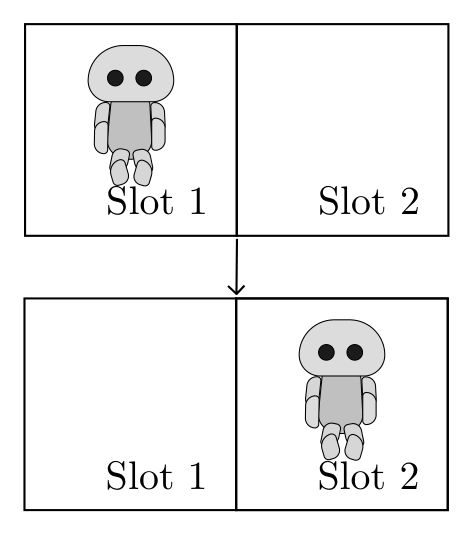
\includegraphics[height=6.0cm]{fig16_2_teleport_cutpaste.png}
    \end{column}
    \begin{column}{0.58\textwidth}
      \small
      \textbf{First form of teleportation}: the agent is cut-and-pasted into
      a new slot. This is essentially the same as \emph{moving the
      position} of the agent -- like a ``wormhole'' teleportation -- where
      only the agent's \emph{location} changes, and there is exactly one
      continuous agent throughout (continuity of existence is preserved).
    \end{column}
  \end{columns}
\end{frame}

\begin{frame}{Figure 16.3: Copy-Paste-and-Delete Teleportation}
  \begin{columns}[c]
    \begin{column}{0.42\textwidth}
      \centering
      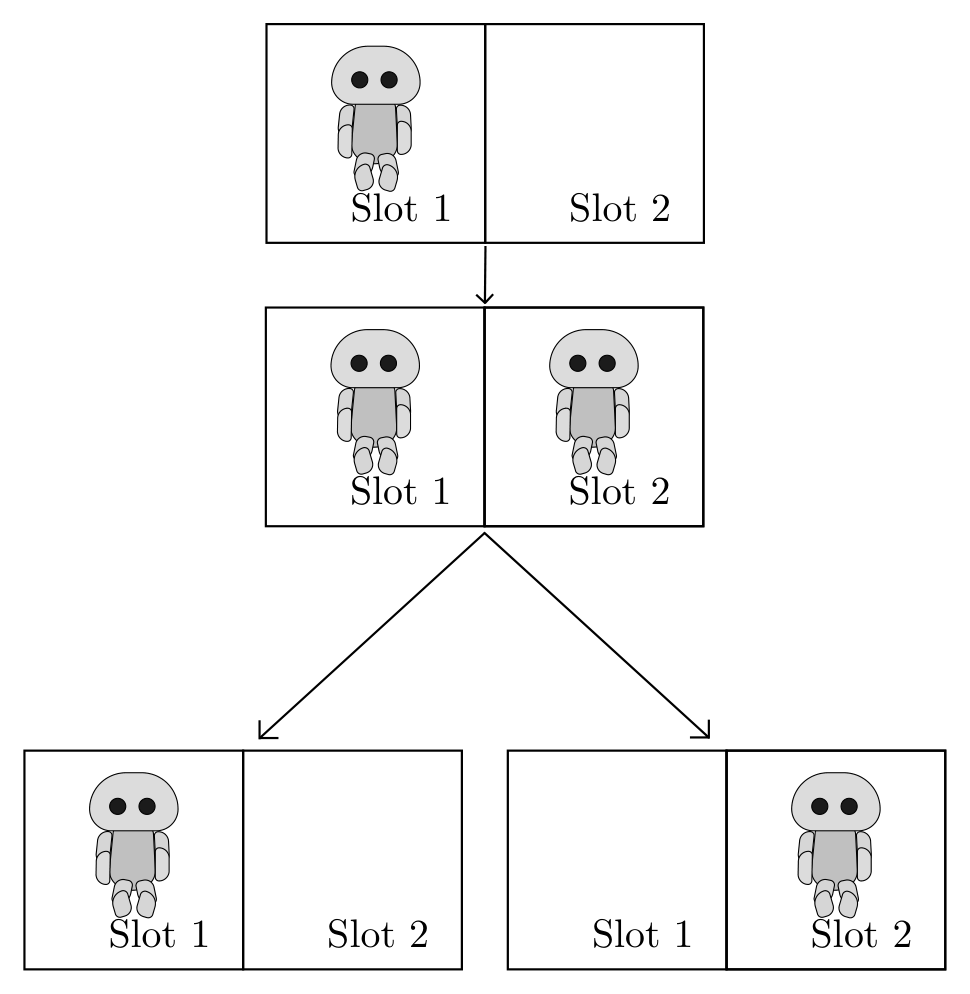
\includegraphics[height=6.0cm]{fig16_3_teleport_copydelete.png}
    \end{column}
    \begin{column}{0.58\textwidth}
      \small
      \textbf{Second form of teleportation}: the agent is first
      \emph{copied} into a new slot; then \emph{one} of the two resulting
      copies is deleted. This mirrors the sci-fi trope (e.g.\ \emph{Star
      Trek}) where an agent is scanned and reconstructed from local
      material at the target location, then the ``original'' is destroyed.
      Unlike cut-and-paste, there is momentarily \emph{two} copies of the
      agent before one is deleted.
    \end{column}
  \end{columns}
\end{frame}

\begin{frame}{Who Chooses to Teleport?}
  \begin{itemize}
    \item In \textbf{both} types of teleportation, a \textbf{copy-centered}
      agent will always choose to teleport, since it values having at least
      one copy of itself receive future observations, and teleporting does
      not reduce that (indeed cloning can only help).
    \item A \textbf{slot-centered} $\mathrm{AI}\mu$ agent will \emph{not}
      teleport, since $\mathrm{AI}\mu$ acts to preserve exactly itself (its
      known slot), and teleporting risks losing its own identity/slot.
    \item A \textbf{slot-centered AIXI} agent, by contrast, \emph{may}
      choose to teleport, precisely because it is uncertain about which
      slot it currently occupies -- teleporting can be informative or
      advantageous under that uncertainty.
  \end{itemize}
  \vspace{0.4em}
  This mirrors an earlier open question in the book about whether AIXI or
  $\mathrm{AI}\mu$ would choose to \emph{self-modify}: the answer depends
  entirely on how the value function is defined, not on some
  environment-independent notion of ``identity.''
\end{frame}

%% ══════════════════════════════════════════════════════════════════════════
\section{16.5 Arguments against AGI}

\begin{frame}{Overview: Arguments against AGI}
  There is a long history of important thinkers arguing that computers will
  never do certain things at all, or as well as humans. Most of these
  arguments, the book argues, break down once they are made fully
  rigorous/formal. We cover four representative arguments:
  \begin{enumerate}
    \item \textbf{Informal arguments of disability} (16.5.1): ``a computer
      could never do $X$.''
    \item \textbf{Chinese room argument} (16.5.2): mimicking intelligence
      is not the same as \emph{understanding} or being conscious.
    \item \textbf{No Free Lunch theorems} (16.5.3): averaged uniformly over
      all problems, all algorithms perform equally (poorly) -- so universal
      solutions (hence AGI) might seem impossible.
    \item \textbf{Penrose--Lucas arguments} (16.5.4): a Gödel-like sentence
      that is true, but that no machine can ever prove is true.
  \end{enumerate}
\end{frame}

\begin{frame}{16.5.1 Informal Arguments of Disability}
  The \emph{argument of disability}: there exist tasks humans can do that
  an AI never can -- play chess, translate languages, read faces, write
  poetry, compose music, hold a conversation, etc.

  \vspace{0.4em}
  \textbf{Historical pattern:} a task once thought impossible for a
  computer is often eventually solved (or attempted with reasonable
  performance) once it is formalized, the right algorithmic approach is
  found, and/or enough compute/training data becomes available:
  \begin{itemize}
    \item Chess was thought unsolvable, until it was (Deep Blue, 1997).
    \item Go, with its enormous branching factor requiring deep intuition,
      was thought unsolvable, until AlphaGo (2016).
    \item Real-time strategy games with huge continuous action spaces and
      only pixel input (\emph{Dota 2}, \emph{Starcraft 2}) were thought
      unsolvable, until they too were mastered.
  \end{itemize}

  \vspace{0.3em}
  \textbf{Moving goalposts:} once a task is solved by AI, it is often no
  longer considered a ``true'' test of intelligence (e.g.\ chess-playing is
  now called mere ``heuristic search'' or ``optimization''). AI-skeptics
  risk converging on the absurd claim that \emph{no} task requires
  intelligence.
\end{frame}

\begin{frame}{16.5.2 The Chinese Room Argument}
  \textbf{Setup} (Searle, 1980): imagine a room with a small input/output
  slot. Questions written in Chinese are inserted; answers (also in
  Chinese) are retrieved. Inside is a person who speaks \emph{no} Chinese,
  but has an instruction book (in English) telling them exactly how to
  match input symbols to output symbols.

  \vspace{0.3em}
  \textbf{Figure 16.4.}
  \begin{center}
    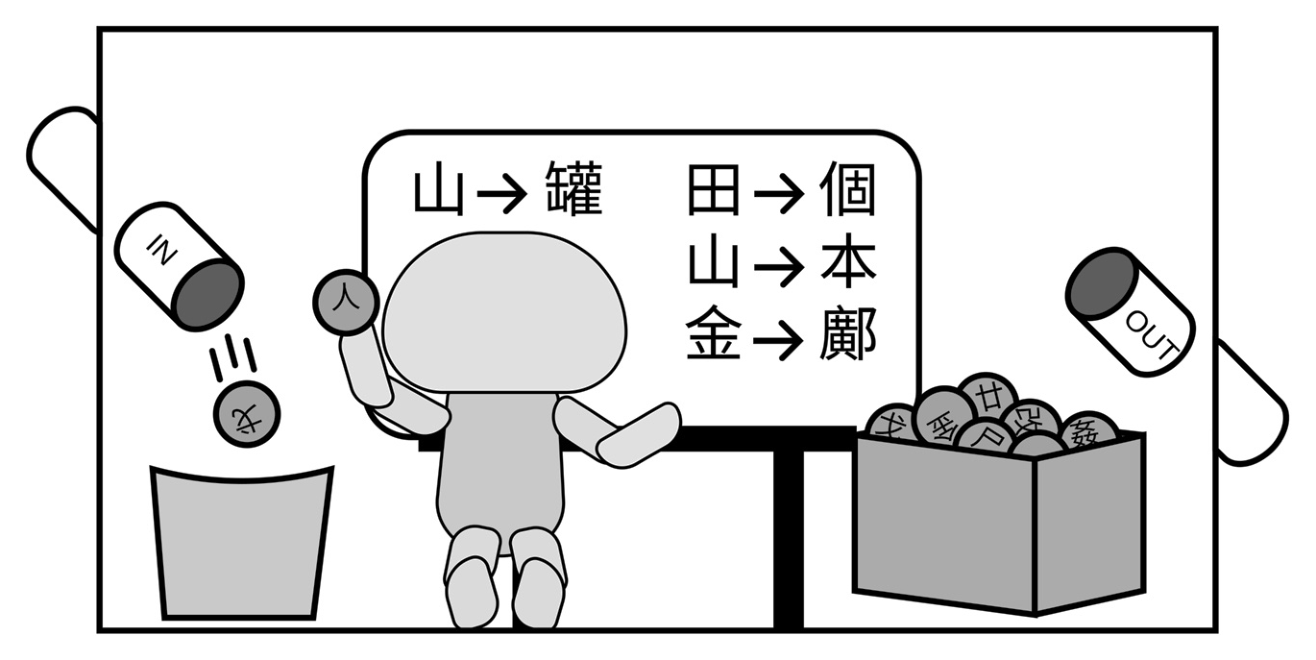
\includegraphics[width=0.52\linewidth]{fig16_4_chinese_room.png}
  \end{center}
  From the outside, the room appears fluent in Chinese. But the person
  inside does not understand a word -- they are mechanically following
  instructions. The argument: an AI, similarly, may just be following a
  ``book of instructions'' without any real understanding.
\end{frame}

\begin{frame}{Chinese Room: A First Counter-Argument}
  \textbf{This does not refute the weak AI hypothesis} (Section 16.3),
  which is the primary hypothesis this book is concerned with: our
  intelligence measure (Section 16.7) is based only on how the agent
  \emph{acts}, not on the internal thought process, nor on whether it is
  conscious.

  \vspace{0.3em}
  \textbf{If we do care about the strong AI hypothesis}, one may argue that
  in the Chinese room setup, the \emph{process of using the book} could
  itself be ascribed intelligence, since it possesses perfect knowledge of
  the meaning of words, characters, and sentences in Chinese -- and
  therefore, on some level, ``understands'' those meanings.
\end{frame}

\begin{frame}{Chinese Room: Further Refutations}
  \textbf{Objecting to the book itself.} A book that lets someone converse
  fluently without \emph{any} understanding could not be a simple
  phrase-book or dictionary. It would need to break input sentences into
  words, look each up, construct a response, and translate back -- so the
  user would need at least \emph{some} understanding of Chinese structure.
  If the user truly had \emph{zero} understanding, the book would need to
  be an astronomically massive lookup table, with a mechanism to search it
  quickly -- and given the exponential (or infinite) number of possible
  sentences, such a book may not even fit in the accessible universe. We
  may reasonably ascribe understanding to whatever process \emph{created}
  such a book.

  \vspace{0.4em}
  \textbf{The neuron analogy.} One could argue human ``understanding'' is
  merely an emergent phenomenon of neurons firing -- a single neuron
  clearly does not understand anything, so (by the same logic) no part of
  the brain understands, so humans do not either. This is absurd from our
  own perspective. \textbf{The fallacy}: assuming a whole cannot have a
  property that none of its parts have individually. No single bolt, nut,
  or rod in a car engine can transport people; only the assembled whole
  can.
\end{frame}

\begin{frame}{16.5.3 No Free Lunch Theorems}
  The \textbf{No Free Lunch (NFL)} theorems state that, averaged uniformly
  over \emph{all} possible problems (in a certain class), every algorithm
  performs equally -- and equally poorly. This is popular among machine
  learners as a justification for domain-specific approaches, and has been
  used to argue against AGI (the ultimate domain-\emph{agnostic} solver).

  \vspace{0.2em}
  NFL is formally a version of what Hume called the \emph{principle of
  uniformity of nature}, which (taken to the extreme) would invalidate all
  inductive reasoning. The theorems are mathematically correct, provided
  their key assumption holds: complete uniformity over problems.

  \begin{block}{Thesis 16.5.1 (Universal $= M$ vs.\ uniform $=$ NFL sampling)}
    \begin{itemize}
      \item The universal distribution $M$ is a \emph{non-dogmatic}
        quantification of Occam's razor -- a cornerstone of science and a
        solution to the induction problem.
      \item The uniform distribution over data is a \emph{dogmatic} prior:
        the belief that the world is pure white noise.
    \end{itemize}
  \end{block}

  \vspace{0.2em}
  \small
  The fallacy: equating ``uniformly distributed problems'' with
  ``uniformly distributed \emph{data}.'' The latter means data is (almost
  surely) white noise, on which induction \emph{must} fail -- but almost
  nobody cares about performing well on pure noise. If instead
  \emph{problems} (programs) are uniformly distributed, induction via a
  universal Turing machine works extremely well, since output strings then
  have a built-in bias toward simplicity.
\end{frame}

\begin{frame}[fragile]{Python: No Free Lunch, Empirically}
  Averaged over \emph{all} possible reward assignments on a tiny search
  space, two very different fixed search algorithms achieve identical
  average performance -- illustrating the NFL theorem directly.
  \begin{lstlisting}[style=pycode]
import numpy as np
rng = np.random.default_rng(0)
n_points, n_functions = 8, 3000
idx = np.arange(n_points)
def best_seen(order, values):
    seen, out = -np.inf, []
    for i in order:
        seen = max(seen, values[i]); out.append(seen)
    return out
avgA = np.zeros(n_points); avgB = np.zeros(n_points)
for _ in range(n_functions):
    values = rng.permutation(n_points).astype(float)  # random problem
    orderA = rng.permutation(n_points)   # Algorithm A: arbitrary traversal
    orderB = idx.copy()                  # Algorithm B: always 0,1,2,...
    avgA += best_seen(orderA, values)
    avgB += best_seen(orderB, values)
avgA /= n_functions; avgB /= n_functions
print("Algorithm A:", np.round(avgA, 3))
print("Algorithm B:", np.round(avgB, 3))
# -> the two rows are (statistically) identical: NFL in action.
  \end{lstlisting}
\end{frame}

\begin{frame}{No Free Lunch: The Resulting Curves Coincide}
  \begin{center}
    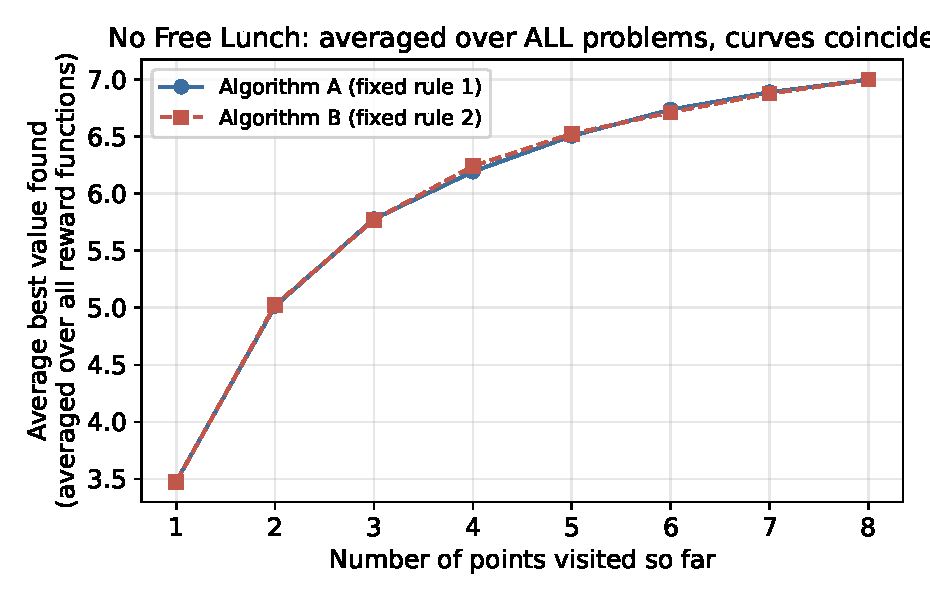
\includegraphics[width=0.55\linewidth]{no_free_lunch}
  \end{center}
  \small
  Averaged over \emph{all} possible reward functions, Algorithm A (a fixed
  ``arbitrary-looking'' traversal) and Algorithm B (the fixed cyclic
  traversal $0,1,2,\ldots$) find, on average, exactly the same best value
  after visiting the same number of points -- neither algorithm is better
  than the other once every problem is equally likely.
\end{frame}

\begin{frame}{16.5.4 The Penrose--Lucas Arguments}
  The \textbf{Penrose--Lucas} argument is effectively an instance of the
  argument from disability (16.5.1), but formal and worth engaging with. It
  claims there exist true logical statements that an AI can never prove,
  but that humans can see are true \emph{by reason} -- a consequence of
  Gödel's incompleteness theorem.

  \vspace{0.3em}
  \textbf{Penrose:} \emph{``The inescapable conclusion seems to be:
  Mathematicians are not using a knowably sound calculation procedure in
  order to ascertain mathematical truth. We deduce that mathematical
  understanding -- the means whereby mathematicians arrive at their
  conclusions with respect to mathematical truth -- cannot be reduced to
  blind calculation!''}

  \vspace{0.3em}
  \textbf{Lucas:} \emph{``Given any machine which is consistent and capable
  of doing simple arithmetic, there is a formula it is incapable of
  producing as being true but which we can see to be true.''}
\end{frame}

\begin{frame}{The Gödel Sentence for AIXI -- and Its Mirror Image}
  \textbf{The claimed Gödel sentence:}
  \begin{center}
    \emph{``AIXI cannot prove that this sentence is true.''}
  \end{center}
  Penrose claims humans see this sentence is obviously true, while AIXI
  cannot prove it.

  \vspace{0.4em}
  \textbf{But we can construct the mirror-image sentence just as easily}:
  \begin{center}
    \emph{``Penrose cannot prove that this sentence is true.''}
  \end{center}
  Now humans who are \emph{not} Penrose, as well as AI systems, can see
  \emph{this} sentence is true (by contradiction: if Penrose could prove it
  true, it would be false). Yet Penrose himself can never prove it.

  \vspace{0.4em}
  \textbf{Conclusion:} although Penrose--Lucas raises an interesting point
  about the logical limits of \emph{any} sufficiently powerful formal
  reasoning system, it is likely irrelevant to AGI: an inability to prove
  every true statement is far too strict a requirement for a definition of
  intelligence -- human mathematicians also have limitations on recognizing
  unprovable truths, and make mistakes. Moreover, to even understand the
  self-referential sentence purely arithmetically, one would need to know
  AIXI's exact source code, and AIXI would need to know its own soundness
  -- something a suitably idealized ``mechanical knower'' provably cannot
  do for itself.
\end{frame}

%% ══════════════════════════════════════════════════════════════════════════
\section{16.6 Arguments for AGI}

\begin{frame}{Overview: Arguments for AGI}
  In contrast to Section 16.5, we now present philosophical and
  \emph{experimental} arguments \emph{for} the eventual possibility (or
  even near-term arrival) of AGI:
  \begin{enumerate}
    \item \textbf{Physical Church-Turing thesis} (16.6.1): intelligent
      hardware (human brains) already exists, so replicating it in machines
      is an \emph{engineering}, not a philosophical, problem.
    \item \textbf{Moore's Law} (16.6.2): computing power has doubled
      roughly every 18 months for a century, and has already surpassed
      naive estimates of raw human-brain compute.
    \item \textbf{AI Progress} (16.6.3): the accelerating, broad track
      record of concrete AI successes across games, vision, language, and
      science.
    \end{enumerate}
\end{frame}

\begin{frame}{16.6.1 The Physical Church-Turing Thesis}
  \begin{block}{Physical Church-Turing Thesis (PCT / Church-Turing-Deutsch principle)}
    \emph{All physical processes are computable.}
  \end{block}

  If \textbf{physicalism} is true (the behaviour of any object is defined
  entirely by its physical properties), then PCT applied to the human mind
  implies that all behaviour of the human mind is computable -- ruling out
  something incorporeal (a ``soul'') being necessary for consciousness to
  work.

  \vspace{0.3em}
  Since the human mind is an example of a physical process, under this
  assumption it is computable, so there \emph{exists} a Turing machine that
  could (in principle) emulate it: scan a human brain, and simulate the
  scan on a computer. The brain fires at only around 200\,Hz, yet performs
  complex tasks -- suggesting it is a slow but highly parallel device, so a
  faithful simulation could likely run much faster than a biological brain,
  appearing \emph{super-humanly} intelligent from the outside (e.g.\
  effectively getting 10 years to think between each sentence of a
  conversation).
\end{frame}

\begin{frame}{Variations of the Physical Church-Turing Thesis}
  \begin{itemize}
    \item \textbf{Extended Church-Turing thesis (ECT):} ``A probabilistic
      Turing machine can \emph{efficiently} simulate any realistic model of
      computation'' (with `efficiently' usually meaning within polynomial
      time).
    \item \textbf{Quantum complexity-theoretic Church-Turing thesis:} the
      quantum analogue -- ``A quantum Turing machine can efficiently
      simulate any realistic model of computation.''
  \end{itemize}

  \vspace{0.4em}
  Even if PCT (or its variants) turned out to be \emph{wrong}, and
  incomputable physical processes were somehow essential for cognition, it
  would be implausible for such processes to occur \emph{only} in human
  brains -- it is more plausible we could build machines harnessing the
  same physics. If the brain turns out to be an efficient quantum computer,
  we could still build AGI on quantum computers -- this would only
  \emph{delay} AGI until the relevant technology matures, not rule it out.
  A caveat: quantum computers are not strictly \emph{more powerful} than
  classical computers (they can be simulated classically); they may only
  be more \emph{efficient} for certain problems (e.g.\ factoring).
\end{frame}

\begin{frame}{16.6.2 Moore's Law}
  \small
  \textbf{Moore's Law}: computing power roughly doubles every 18 months (a
  faster pace than Moore's original yearly estimate), and this trend has
  held up remarkably well since inception.
  \begin{center}
    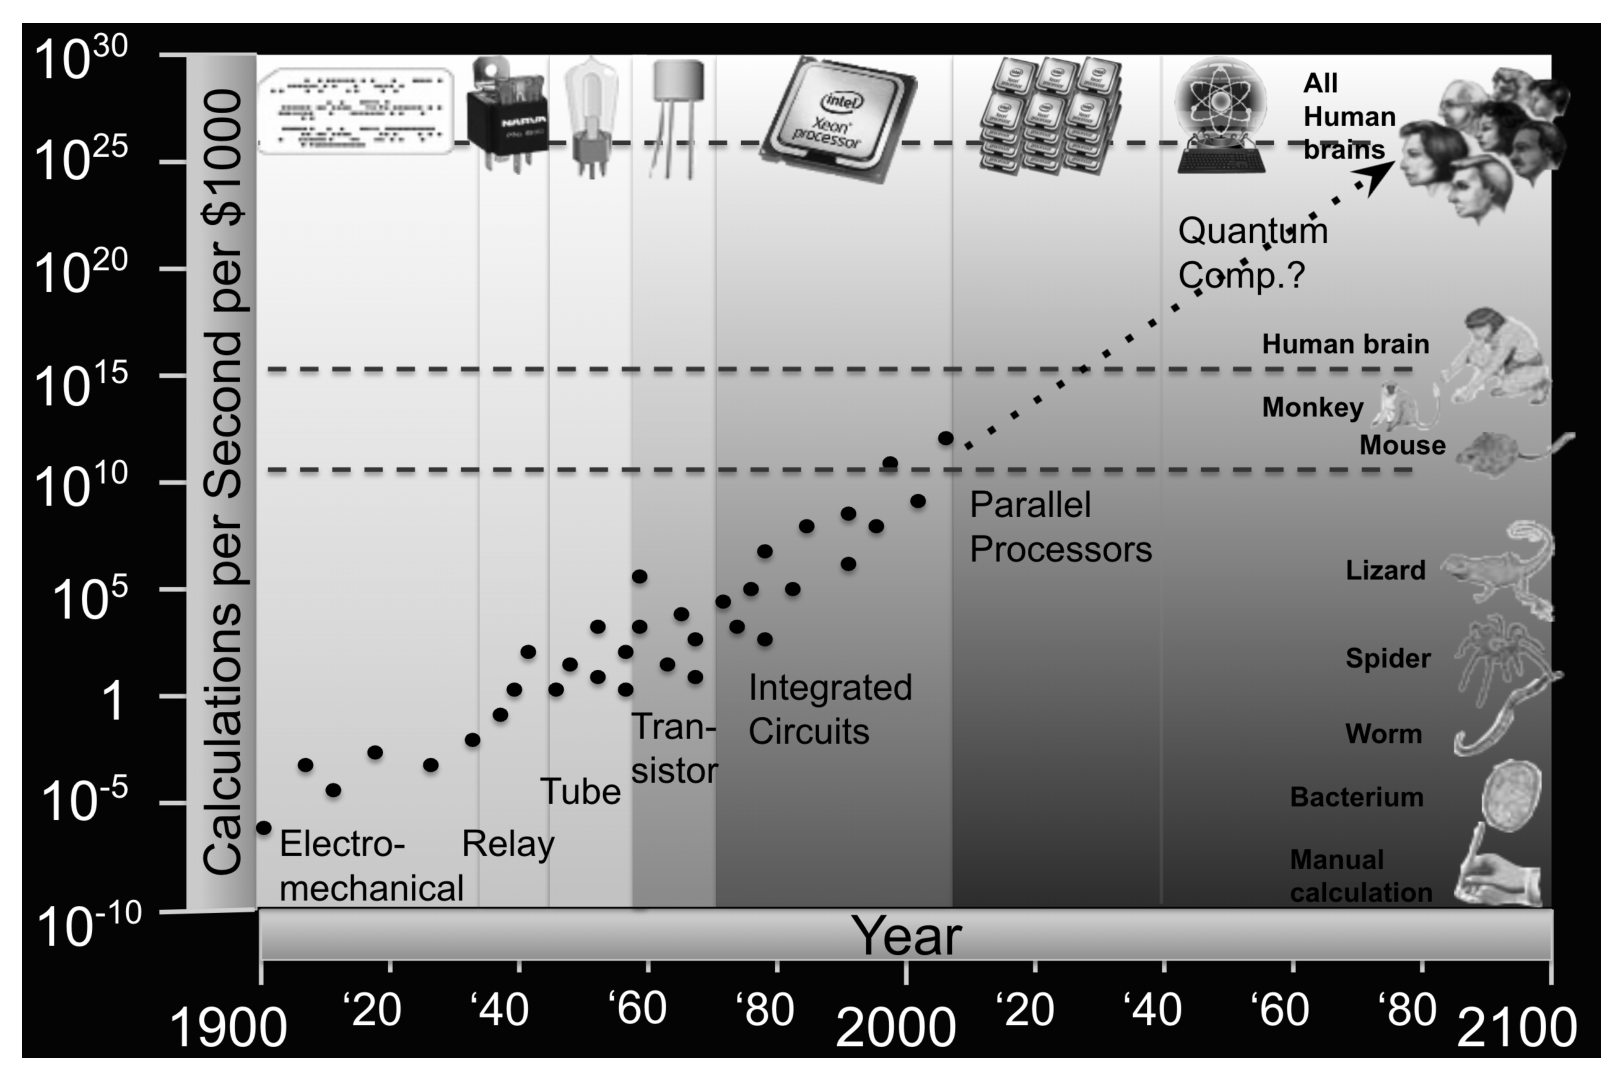
\includegraphics[height=5.6cm]{fig16_5_moore_law.png}
  \end{center}
  {\scriptsize Figure 16.5: computing power (calculations per second per
  \$1000) vs.\ year, log scale, vs.\ estimated compute of biological brains.}
\end{frame}

\begin{frame}{Moore's Law and the Path to AGI}
  Global computing power has grown exponentially to the point of already
  exceeding estimates of raw human-brain compute (roughly $10^{17}$ logical
  operations per second). Assuming PCT, it would already be
  \emph{theoretically} possible to simulate a human mind computationally --
  but having enough raw operations-per-second is not sufficient:
  \begin{itemize}
    \item little is known about \emph{how} the brain actually operates at
      sufficient fidelity to simulate;
    \item the technology to \emph{scan} a brain at sufficient resolution
      does not yet exist;
    \item the computational overhead of simulation may make brain
      simulation intractable for a few more decades of Moore's law, even if
      possible in principle.
  \end{itemize}
  It was predicted in 2016 that the classical doubling trend would slow
  around 2020--2025, but the (possible) rise of accessible quantum
  computers could provide a further computational leap analogous to the
  classical one.
\end{frame}

\begin{frame}{16.6.3 AI Progress: Perception and Language}
  The single strongest piece of evidence for the eventual possibility of
  AGI is arguably the breadth of success AI has already achieved,
  especially since the deep learning era:
  \begin{itemize}
    \item \textbf{Computer vision}: extracting information from images;
      convolutional neural networks (CNNs) exceed human performance on many
      subproblems; \emph{ResNet} uses skip connections to train very deep
      networks; \emph{NeRF} represents 3D scenes with a neural network
      mapping position/viewing-angle to colour.
    \item \textbf{Speech recognition}: transcribing speech to text -- now
      an end-to-end deep-learning task, nearly (but not fully) solved.
    \item \textbf{Machine translation \& NLP}: from the 1960s chatbot
      \emph{Eliza}, to \emph{IBM Watson} winning \emph{Jeopardy!} against
      human champions in 2011, to modern Transformer-based systems that can
      write articles indistinguishable from human writing.
  \end{itemize}
\end{frame}

\begin{frame}{AI Progress: Science, LLMs, and Multimodal Models}
  \begin{itemize}
    \item \textbf{AlphaFold} (DeepMind): predicts 3D protein structure from
      amino-acid sequence with accuracy comparable to costly experimental
      methods -- a landmark for AI-assisted science.
    \item \textbf{GPT-4 Turbo} (OpenAI, Nov.\ 2023): a decoder-only
      Transformer, scoring 90th percentile on the Bar Exam, and processing
      both visual and textual input. The key architectural ingredient is
      the \textbf{attention mechanism}, letting the model weigh the
      relative importance of every other position in a sequence, and
      allowing parallel (rather than strictly sequential) processing during
      training.
    \item \textbf{CLIP} (Contrastive Language-Image Pre-Training):
      jointly trains a vision Transformer and a text Transformer so that
      matching (image, caption) pairs map to nearby embedding vectors --
      producing a semantically meaningful representation used as input to
      many other models.
  \end{itemize}
\end{frame}

\begin{frame}{Generative AI and Diffusion Models}
  \textbf{Diffusion models} learn a complex data distribution (e.g.\ over
  images of animals) by defining a \textbf{diffusion process}: starting
  from a real datapoint $x_1 = x$, each successive term
  $x_{t+1} = x_t + \varepsilon_t$ adds a small amount of Gaussian noise
  $\varepsilon_t$ (varepsilon, a random perturbation) according to a
  schedule, so that after $T$ steps $x_T$ looks like pure random noise
  (analogous to a drop of dye diffusing in water, driven by entropy).

  \vspace{0.3em}
  \textbf{Generation}: the model learns to \emph{undo} this process --
  de-noise $x_{t+1}$ back towards $x_t$ -- so that starting from pure random
  noise and repeatedly applying the learned de-noising step produces a
  brand-new, realistic sample. \emph{Latent} diffusion models first
  compress images into a smaller, semantically meaningful feature space
  (using e.g.\ a U-net and CLIP), making generation far more efficient.
  Applications include image generation/upscaling, video, music, and 3D
  mesh generation.
\end{frame}

\begin{frame}[fragile]{Python: A Numeric Forward-Diffusion Demo}
  \begin{lstlisting}[style=pycode]
import numpy as np
rng = np.random.default_rng(1)
n, T = 200, 5
t_axis = np.linspace(0, 4*np.pi, n)
x0 = np.sin(t_axis) + 0.3*np.sin(3*t_axis)      # a clean "signal"
alphas = np.linspace(0, 1, T) ** 1.6            # noise-fraction schedule
for step, a in enumerate(alphas):
    xt = np.sqrt(1 - a) * x0 + np.sqrt(a) * rng.normal(size=n)
    sig_var = np.var(np.sqrt(1 - a) * x0)
    noise_var = np.var(np.sqrt(a) * rng.normal(size=n))
    print(f"step {step}: alpha={a:.2f}  sig-var={sig_var:.3f}  noise-var={noise_var:.3f}")
# As alpha: 0 -> 1, sig-var shrinks to 0, noise-var grows to 1:
# x0 (clean sine wave) morphs smoothly into x_T (pure Gaussian noise).
  \end{lstlisting}
  \begin{center}
    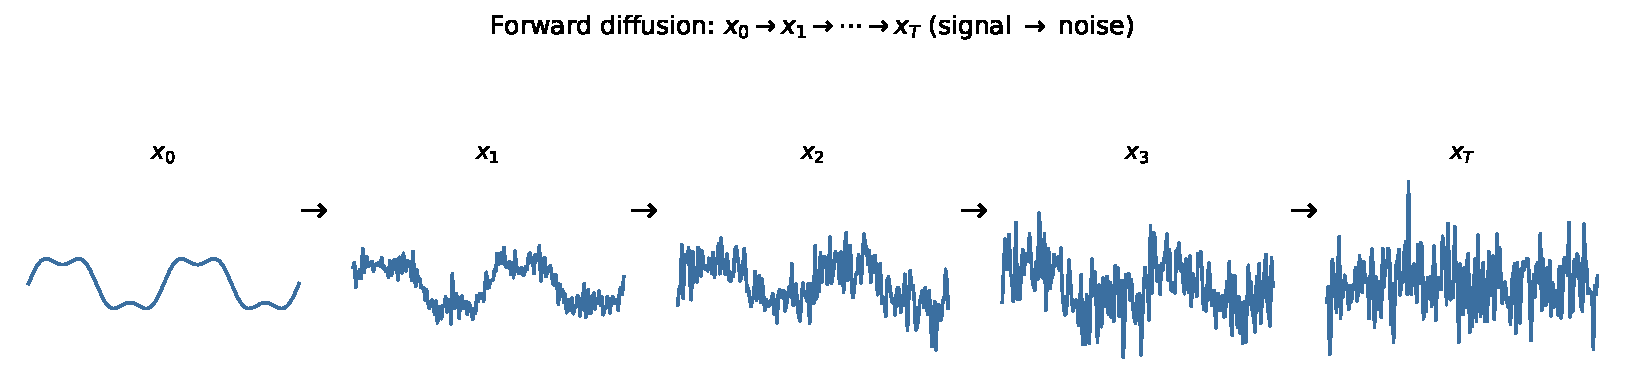
\includegraphics[width=0.75\linewidth]{diffusion_schematic}
  \end{center}
\end{frame}

\begin{frame}{AI Progress: Games as a Proxy for Intelligence}
  Games are popular because the goal, action space, and dynamics are
  well-defined, with communities of high-level human players to compare
  against. Notable milestones:
  \begin{itemize}
    \item \textbf{Checkers} (1959): early reinforcement learning beats its
      creator.
    \item \textbf{TD-gammon} (1995): self-play + TD learning reaches
      master-level Backgammon.
    \item \textbf{Deep Blue} (1997): defeats world chess champion Garry
      Kasparov using custom hardware and a hand-tuned evaluation function.
    \item \textbf{DQN} (2015): masters a large collection of Atari games at
      human level.
    \item \textbf{AlphaGo} (2016): Monte-Carlo tree search $+$ deep neural
      networks defeat world Go champion Lee Sedol.
  \end{itemize}
\end{frame}

\begin{frame}[allowframebreaks]{AI Progress: Games (continued)}
  \begin{itemize}
    \item \textbf{AlphaStar} (2019): combines supervised learning and RL to
      rank in the top 0.2\% of \emph{StarCraft} players.
    \item \textbf{Pluribus} (2019): a superhuman poker agent, using Monte
      Carlo counterfactual regret minimization plus self-play, beating
      elite professional poker players.
    \item \textbf{MuZero} (2020): learns \emph{Go}, chess, \emph{Shogi},
      and Atari games using Monte Carlo Tree Search and self-play, with
      \emph{no} prior domain knowledge -- exceeding AlphaGo.
    \item \textbf{Agent57} (2020): a deep RL agent achieving human-level
      performance across \emph{all} 57 games of the Arcade Learning
      Environment (ALE) benchmark.
    \item \textbf{Cicero} (2022): an LLM tuned with RL, ranked in the top
      10\% of online \emph{Diplomacy} players -- a game requiring tactical
      decision-making \emph{and} negotiation with other (human) players.
    \item \textbf{Gato} (2022): a single multimodal agent excelling at a
      large collection of games, robotics, vision, and language tasks
      simultaneously.
  \end{itemize}
\end{frame}

\begin{frame}{The Role of Language in Intelligence}
  Language models such as GPT-3 and GPT-4 have been shown to generalize
  well beyond pure language tasks -- playing chess, writing code, and
  passing theory-of-mind tests. Language can act as an efficient compression
  or coding scheme for knowledge, but there remain concepts that are
  fundamentally hard to convey \emph{only} through language (e.g.\ a
  detailed image) -- as the saying goes, ``a picture is worth a thousand
  words.''
\end{frame}

%% ══════════════════════════════════════════════════════════════════════════
\section{16.7 Intelligence}

\begin{frame}{What Is Intelligence?}
  Researchers have struggled for decades to define intelligence precisely.
  Common informal themes: the ability to solve a \emph{wide class} of
  problems, display creativity/reasoning/deduction, and acquire and process
  \emph{new} knowledge.

  \vspace{0.3em}
  Crucially, we want a system that is good at \emph{all} tasks (including
  ones it has never seen before), rather than a collection of narrow,
  built-in skills -- this is the notion of \textbf{general} intelligence
  this chapter tries to formalize.
\end{frame}

\begin{frame}{16.7.1 Legg--Hutter (LH) Intelligence: Informal}
  Synthesizing many definitions from psychology, philosophy, computer
  science, and neuroscience, Legg and Hutter proposed:

  \begin{block}{Legg--Hutter (LH) Intelligence (informal)}
    \emph{Intelligence measures an agent's ability to achieve goals in a
    wide range of environments.}
  \end{block}

  This captures performing well across a \emph{wide class} of problems,
  rather than excelling at one narrow task: a chess bot may play chess
  superhumanly, but cannot fill out tax forms, load a dishwasher, or
  compose poetry. It also excludes a ``wise hermit'' intelligence that
  thinks all day but takes no action affecting its environment -- such an
  agent would be indistinguishable from an unintelligent one and serve no
  useful purpose. Requiring the agent to \emph{achieve goals} captures this,
  while remaining agnostic to the strong-AI hypothesis (Section 16.3):
  only the agent's actions matter, not its internal state.
\end{frame}

\begin{frame}{16.7.2 Other Intelligence Tests and Measures (I)}
  \begin{itemize}
    \item \textbf{Raven test}: recognize a pattern in a sequence of
      geometric images and choose the missing piece. Narrow (pattern
      recognition), but many problems can be reframed as sequence
      prediction, so it is not entirely disconnected from general
      intelligence.
    \item \textbf{Turing test}: an interrogator chats (text only) with both
      a human and an AI; the AI ``passes'' if the interrogator cannot
      reliably tell them apart. Too strict: it tests mimicry of \emph{human
      idiosyncrasy} (even including deliberately misspelled words) rather
      than intelligence -- a genuinely intelligent alien species would
      likely \emph{fail} it, not because it is unintelligent, but because it
      lacks familiarity with human culture and language. It is also purely
      binary (pass/fail), not a graded score.
    \item \textbf{Loebner prize} (1991--2019): a cash prize for the most
      human-like chatbot (judged by a human panel); the top \$100{,}000
      prize (for fooling a judge completely) was never claimed.
  \end{itemize}
\end{frame}

\begin{frame}{16.7.2 Other Intelligence Tests and Measures (II)}
  \begin{itemize}
    \item \textbf{Hutter prize}: a cash prize for how far
      \texttt{enwik9} (a 1GB sample of Wikipedia) can be losslessly
      \emph{compressed}. Motivation: compression is closely linked to
      intelligence -- an ``intelligent'' compressor finds and exploits
      patterns/regularities in the data, using them to predict (and hence
      compress) further.
    \item \textbf{Chollet's measure}: views intelligence as the ability to
      \emph{adapt and generalize} to novel situations by recognizing
      patterns and re-using previously learned knowledge -- emphasizing
      transfer of knowledge across domains, in contrast to traditional IQ
      tests or task-specific performance measures.
    \item \textbf{AI-Complete} (informal, by analogy with NP-Complete):
      problems for which \emph{any} algorithm solving them must be
      generally intelligent -- e.g.\ fluent human-level translation,
      automatic peer review of research papers, or proving prize-worthy
      mathematical theorems.
  \end{itemize}
\end{frame}

\begin{frame}{16.7.3 Formalizing the LH-Intelligence Measure: Design Choices}
  We want to define general intelligence as a \emph{weighted average} of
  how well an agent achieves ``the goal'' across a large class of
  environments. This raises several design questions:

  \begin{itemize}
    \item \textbf{Goals}: too simple a goal makes every agent ``intelligent
      by definition''; too internal a goal lets the agent cheat by picking
      an easy target. Solution: the goal is communicated to the agent
      \emph{by the environment}, via rewards, within the standard cybernetic
      agent-environment model -- the goal is always maximizing the sum of
      rewards (the \emph{reward hypothesis}).
    \item \textbf{Balance}: should easy environments (where any agent does
      well) dominate the average? No -- we want to penalize agents heavily
      for failing simple environments, but only lightly for failing
      difficult ones (since few agents can succeed there at all).
  \end{itemize}
\end{frame}

\begin{frame}{16.7.3 Formalizing LH-Intelligence: Universality and Balance}
  \textbf{Universality (avoiding a discount-rate parameter).} Optimal
  behaviour depends on how far-sighted the agent is (its discount factor
  $\gamma$, gamma). To avoid making intelligence dependent on this
  arbitrary choice, and to prevent some environments dominating just by
  offering disproportionately large rewards, we restrict to
  \textbf{reward-summable} environments: those where the total reward
  received can never exceed $1$.

  \begin{block}{Bounded value function}
    \[
      V^\pi_\rho \;:=\; \E^\pi_\rho\!\left[\sum_{i=1}^{\infty} r_i\right] \;\le\; 1
    \]
    for any policy $\pi$ and environment $\rho$ (rho). $\E^\pi_\rho$ is the
    expectation of the total reward $\sum r_i$ collected when policy $\pi$
    acts in environment $\rho$; bounding it by 1 removes the need for
    discounting altogether -- how quickly an environment ``spends'' its
    limited reward budget determines whether short- or long-term planning
    is required, rather than an externally imposed discount rate.
  \end{block}
\end{frame}

\begin{frame}{16.7.3 Formalizing LH-Intelligence: Environment Class and Weighting}
  \textbf{Environment class $\Mc$}: chosen to be as general as possible --
  \emph{any} computable stochastic environment. Incomputable environments
  are excluded, since there would be no way to even accurately predict
  what percepts/rewards they would return (and the physical Church-Turing
  thesis, Section 16.6.1, makes considering them unnecessary anyway).

  \vspace{0.3em}
  \textbf{Weighting}: not all environments are equally difficult. We use
  Kolmogorov complexity $K$ as a proxy for difficulty: environments with a
  short description (in the Kolmogorov sense) are expected to be easier to
  perform well in, since the agent has fewer bits to learn to identify the
  true environment. Hence the natural weighting is the \textbf{universal
  prior} $2^{-K(\mu)}$ over environments $\mu$ -- the very same prior used
  for universal induction in Section 16.1. This choice makes the
  intelligence measure itself an embodiment of Occam's razor.
\end{frame}

\begin{frame}{16.7.4 Legg--Hutter (LH) Intelligence: Formal Definition}
  \begin{block}{Definition 16.7.1 (Legg--Hutter intelligence)}
    The intelligence $\Upsilon(\pi)$ (capital upsilon) of a policy $\pi$ is
    the undiscounted value function of $\pi$, averaged over all
    reward-summable computable stochastic environments $\Mc$, weighted by
    the Kolmogorov complexity of each environment:
    \[
      \Upsilon(\pi) \;:=\; \sum_{\nu \in \Mc} 2^{-K(\nu)}\, V^\pi_\nu(\epsilon)
    \]
    where $V^\pi_\nu(\epsilon) = \E^\pi_\nu\!\left[\sum_{t=1}^\infty
    r_t\right]$ is the expected total reward earned by $\pi$ in environment
    $\nu$, starting from the empty history $\epsilon$.
  \end{block}
  \small
  In words: intelligence is the weighted average of how well $\pi$ performs
  across every computable, reward-summable environment $\nu$, where
  simpler environments (lower $K(\nu)$) count for more.
\end{frame}

\begin{frame}{Theorem: AIXI Maximizes LH Intelligence}
  \begin{block}{Theorem 16.7.2 (AIXI maximizes LH intelligence)}
    \[
      \pi^{\mathrm{AIXI}} := \pi^*_\xi = \arg\max_\pi \Upsilon(\pi), \qquad
      \overline{\Upsilon} := \max_\pi \Upsilon(\pi) = \Upsilon(\pi^{\mathrm{AIXI}})
    \]
  \end{block}
  Here $\pi^{\mathrm{AIXI}} = \pi^*_\xi$ is the (undiscounted) Bayes-optimal
  policy that maximizes expected value under the universal mixture $\xi$
  (xi); $\overline{\Upsilon}$ denotes the highest LH-intelligence score any
  policy can achieve.

  \vspace{0.4em}
  AIXI is precisely this Bayes-optimal agent from earlier chapters, and it
  achieves the \emph{maximum possible} LH-intelligence score
  $\overline{\Upsilon}$. The gap $\overline{\Upsilon} - \Upsilon(\pi)$
  measures exactly how far any other agent $\pi$ falls short of the
  theoretical optimum.
\end{frame}

\begin{frame}{Why This Definition Is a Good One}
  The Legg--Hutter definition is claimed to be:
  \begin{itemize}
    \item \textbf{valid} (well-motivated by the informal definition),
    \item \textbf{meaningful} (high-scoring agents do well in most simple
      and many complex environments),
    \item \textbf{informative} (gives a graded numerical score, not
      pass/fail),
    \item \textbf{wide-range} (orders everything from random policies to
      super-intelligent AIXI),
    \item \textbf{general} (covers the entire class of computable
      environments, the largest class we could ever need),
    \item \textbf{unbiased} towards culture/language (unlike the Turing
      test), \textbf{fundamental} (built from computability, complexity,
      and information theory), and \textbf{objective}
      (\textbf{non-anthropocentric}: unlike most tests, it does not measure
      relative to how \emph{humans} behave -- a super-intelligent agent with
      zero cultural knowledge would fail the Turing test yet still score
      very highly here).
  \end{itemize}
\end{frame}

\begin{frame}{Drawbacks of LH Intelligence}
  \begin{itemize}
    \item It is \textbf{incomputable}, since it depends on Kolmogorov
      complexity $K$, which is itself incomputable. Approximations are
      needed in practice (Section 16.7.5).
    \item There is a hidden parameter: the choice of the reference
      \textbf{universal Turing machine} $U$ used to define $K$. There is
      no known ``canonical'' choice, and this has been an open problem in
      algorithmic information theory since its inception -- some choices
      of $U$ can even lead to nonsensical intelligence rankings.
    \item One could weaken the environment class to something computable,
      like (partially observable) Markov decision processes, replacing the
      incomputable weight $2^{-K(\mu)}$ with a computable substitute.
  \end{itemize}
\end{frame}

\begin{frame}{16.7.5 Approximations of Intelligence: AIQ}
  Practical psychometric tests (Stanford-Binet, Wechsler, Raven, etc.) are
  not \emph{general enough} to be true intelligence tests -- they capture
  memory, reasoning, pattern-recognition, etc.\ separately.

  \vspace{0.3em}
  \textbf{Artificial Intelligence Quotient (AIQ)} approximates
  $\Upsilon(\pi)$ via \emph{sampling}: environments/programs $p$ are sampled
  according to $2^{-\ell(p)}$ ($\ell(p)$ = program length), which
  approximates the simplicity weighting $2^{-K(\mu)}$ (since $K(p) \approx
  \ell(p)$ for most short programs $p$). The AIQ estimator is:
  \begin{block}{AIQ estimator}
    \[
      \hat\Upsilon(\pi) \;:=\; \frac{1}{N}\sum_{i=1}^{N} \hat V^\pi_{p_i}
    \]
    where $\hat V^\pi_{p_i} = \sum_t r_t$ is the empirical return of $\pi$
    on the $i$-th sampled program $p_i$, and $N$ is the number of sampled
    programs. On average, $\hat V^\pi_{p_i}$ equals the true expected
    return $\E^\pi_{p_i}[\sum_t r_t]$.
  \end{block}
  A \textbf{BrainFuck (BF)} interpreter is used as the reference machine: an
  esoteric but Turing-complete language with only 8 symbols, chosen because
  it is simple, unbiased (no built-in domain knowledge), and produces very
  short programs for simple environments.
\end{frame}

\begin{frame}[fragile]{Python: A Toy LH-Intelligence / AIQ Worked Example}
  \begin{lstlisting}[style=pycode]
import numpy as np

# --- (a) Toy LH-intelligence: weighted sum over 5 environments ---
weights = np.array([0.50, 0.25, 0.125, 0.0625, 0.0625])   # ~ 2^-K(nu), nu=1..5
weights /= weights.sum()
general_agent = np.array([0.90, 0.85, 0.75, 0.65, 0.55])   # V^pi_nu for pi_1
narrow_agent  = np.array([0.05, 0.05, 0.05, 0.05, 0.95])   # V^pi_nu for pi_2

upsilon_general = float(np.sum(weights * general_agent))
upsilon_narrow  = float(np.sum(weights * narrow_agent))
print(f"Upsilon(general) = {upsilon_general:.3f}")   # 0.828
print(f"Upsilon(narrow)  = {upsilon_narrow:.3f}")     # 0.106

# --- (b) Toy AIQ: sampling-based estimator, converging as N grows ---
rng = np.random.default_rng(42)
N = 4000
lengths = rng.geometric(p=0.15, size=N)                 # program lengths ~ 2^-l(p)
true_mean = 1.0 / (1.0 + 0.15 * lengths)                 # simpler => higher value
values = np.clip(true_mean + rng.normal(scale=0.15, size=N), 0, 1)
running_avg = np.cumsum(values) / np.arange(1, N + 1)
print(f"AIQ estimate after N={N}: {running_avg[-1]:.3f}")
  \end{lstlisting}
  \textbf{Takeaway:} the general agent has far higher LH-intelligence
  $\Upsilon$ despite \emph{never} being the best in any single environment
  -- breadth, weighted by simplicity, is what the measure rewards.
\end{frame}

\begin{frame}{Atari (ALE) as a Practical Intelligence Measure}
  The \textbf{Arcade Learning Environment (ALE)}, a large collection of
  Atari 2600 games, is a popular practical intelligence proxy: doing well
  across \emph{many} different games is a weak form of general
  intelligence. Deep Q-Networks (DQN) were the first major success; later
  agents such as Agent-57 outperformed humans on all 57 ALE games.

  \vspace{0.3em}
  A handful of games (\emph{Skiing}, \emph{Private Eye}, \emph{Pitfall},
  and especially \emph{Montezuma's Revenge}) remain very hard for most
  agents, because they combine three notoriously difficult RL problems:
  \begin{itemize}
    \item \textbf{Exploration-exploitation trade-off}: balancing learning
      more about the environment vs.\ exploiting what is already known.
    \item \textbf{Long-term credit-assignment problem}: rewards only arrive
      long after the actions that caused them.
    \item \textbf{Partial observability}: the current percept does not
      contain everything needed to determine what happens next.
  \end{itemize}
  Interestingly, agent performance on a carefully chosen subset of just 5
  Atari games has been shown to be already indicative of average
  performance across \emph{all} ALE games.
\end{frame}

\begin{frame}{Solving One Very General Problem}
  Throughout the chapter, ``intelligence'' has meant good performance
  across a \emph{wide class} of (typically simpler) environments. An
  alternative is to consider one, single, very \emph{general}
  environment requiring a large skill set -- e.g.\ a self-driving car
  delivering passengers, which requires computer vision, path-finding,
  object detection/avoidance, and trade-offs between comfort, safety, and
  speed.

  \vspace{0.3em}
  Interestingly, an agent that does well \emph{only} in such a broad, single
  environment, but poorly elsewhere, will still have \textbf{low}
  LH-intelligence $\Upsilon$: a single very general environment
  $\mu_{\text{general}}$ still only gets one (typically small) universal
  prior weight $2^{-K(\mu_{\text{general}})}$ in the sum defining
  $\Upsilon(\pi)$.
\end{frame}

%% ══════════════════════════════════════════════════════════════════════════
\section{16.8 Deep Learning}

\begin{frame}{From ``Is AGI Possible?'' to ``When Will AGI Arrive?''}
  With the rise of increasingly general and powerful Large Language Models
  (LLMs), the conversation has shifted from \emph{whether} AGI is possible
  to \emph{when} it will arrive, and whether current systems already count
  as (proto-)AGI.

  \vspace{0.3em}
  \textbf{Key claim of this section:} the language-modelling path to AGI is
  \emph{not} in opposition to Universal Artificial Intelligence -- it is
  arguably an \textbf{approximation} of the universal Bayesian mixture
  $\xi$ (xi) that AIXI uses. LLMs are trained on huge corpora of text with
  the goal of minimizing \textbf{cross-entropy loss} (a measure of how
  surprised the model is by the next token). To minimize this loss
  efficiently, the model must build an internal representation of the
  knowledge in its training data -- much like a data \textbf{compressor}
  does. As stated earlier in the book: \emph{compression is prediction},
  and Kolmogorov complexity / Solomonoff induction are the theoretical
  ``ultimate'' compressors/predictors.
\end{frame}

\begin{frame}{LLMs, Planning, and MC-AIXI}
  LLMs alone are not complete reinforcement-learning/AI agents, but recent
  work augments them in ways that mirror this book's own extensions of
  Solomonoff induction:
  \begin{itemize}
    \item \textbf{Reasoning-via-Planning (RAP)} augments an LLM with
      planning methods, mirroring how \textbf{MC-AIXI} (Chapter 7 / 12)
      augments Solomonoff induction with Monte Carlo Tree Search (MCTS).
    \item \textbf{In-context learning} (an LLM's ability to adapt its
      behaviour from examples given in its prompt, without updating its
      weights) can be viewed as a form of \textbf{Bayesian inference} --
      and it has been shown that Transformers, when trained on suitably
      algorithmic data, can approximate Solomonoff induction directly.
    \item \textbf{RLHF} (Reinforcement Learning from Human Feedback) is a
      crude form of RL -- essentially using a horizon of just 1 step,
      trained on a model of human preferences/values as a reward proxy.
    \item \textbf{Tree-of-Thought (ToT)}, a search/planning controller
      layered on top of an LLM, corresponds to \textbf{expectimax
      planning}/tree search; combined with in-context learning (the
      analogue of Solomonoff induction here), this yields something like an
      LLM version of MC-AIXI.
  \end{itemize}
\end{frame}

\begin{frame}{What Is Still Missing from LLMs, Relative to AIXI?}
  At the time of writing, LLMs are \textbf{not} AGI on their own. What would
  bring them closer to AIXI?
  \begin{itemize}
    \item \textbf{Long-horizon value functions.} RLHF trains on a horizon
      of essentially 1 step; learning a value function over much longer
      horizons would let models plan and reason at length, rather than
      react token-by-token.
    \item \textbf{New architectures, scaffolding, or controllers} around
      the base model (e.g.\ explicit search/planning modules, or tool use)
      to add the missing long-horizon planning capability.
    \item \textbf{Memory / continual learning.} Current LLMs largely lack a
      good mechanism to store, recall, and learn from past experience
      beyond their fixed context window. Possible directions: an explicit
      external memory controller, or continual learning that compiles
      short-term in-context experience into long-term (in-weight) memory --
      the latter would be closest in spirit to Solomonoff induction, which
      learns continuously and without a fixed context limit.
  \end{itemize}
  AIXI, by contrast, learns continuously, plans at arbitrarily long
  horizons, and handles arbitrary (multimodal) inputs/outputs by
  construction -- serving as the gold-standard \emph{direction} to aim for
  when designing the next generation of LLMs, towards AGSI.
\end{frame}

\begin{frame}[fragile]{Python: Compression Is Prediction}
  A concrete numeric illustration of ``compression is prediction'': a
  \emph{predictable} (structured) sequence compresses far better than a
  \emph{random} one of the same length, exactly as an ideal Solomonoff-style
  predictor would exploit.
  \begin{lstlisting}[style=pycode]
import zlib, math
import numpy as np
rng = np.random.default_rng(0)

n = 20000
structured = (bytes([65 + (i % 4) for i in range(n)]))     # "ABCDABCDABCD..."
random_bytes = bytes(rng.integers(0, 256, size=n, dtype=np.uint8))

for name, data in [("structured (period-4 pattern)", structured),
                    ("random bytes", random_bytes)]:
    compressed = zlib.compress(data, level=9)
    ratio = len(compressed) / len(data)
    bits_per_symbol = 8 * ratio
    print(f"{name:32s}: raw={len(data)}B compressed={len(compressed)}B "
          f"ratio={ratio:.4f} ~{bits_per_symbol:.3f} bits/symbol")
# structured -> tiny fraction of its size (~0.02 bits/symbol);
# random     -> barely compresses at all (~8 bits/symbol = true entropy).
  \end{lstlisting}
\end{frame}

%% ══════════════════════════════════════════════════════════════════════════
\section{16.9 Conclusion}

\begin{frame}{Towards Artificial General Super Intelligence (AGSI)}
  The construction of a truly intelligent system able to act beyond human
  capacity in most areas -- \textbf{Artificial General Super Intelligence
  (AGSI)} -- is one of the most ambitious problems of our time. If achieved,
  it represents the entering of a new era for humanity, and perhaps the
  last invention we ever need to make.

  \vspace{0.4em}
  This book has provided the tools needed to understand and extend the
  \textbf{Universal Artificial Intelligence} approach to this problem --
  from its theoretical and safety/philosophical foundations, to the best
  currently implementable approximations (MC-AIXI, CTW, and beyond).
\end{frame}

\begin{frame}{Chapter Summary}
  \begin{itemize}
    \item \textbf{16.1} Universal induction rests on solid philosophical
      ground: Epicurus, Occam, and Bayes combine into a single formula,
      $w^U_\nu = 2^{-K(\nu)}$.
    \item \textbf{16.2--16.3} Consciousness, free will, and moral status
      remain open, but a pragmatic stance: if these properties are useful
      for acting intelligently, expect them to emerge in AIXI-like agents.
    \item \textbf{16.4} Whether AIXI-like agents self-replicate or teleport
      depends entirely on how their value function is defined (copy- vs.\
      slot-centered).
    \item \textbf{16.5--16.6} Most informal arguments against AGI break
      down under formal scrutiny; arguments for AGI (PCT, Moore's Law, and
      especially concrete AI progress) are compelling and mounting.
    \item \textbf{16.7} The Legg--Hutter measure $\Upsilon(\pi)$ formalizes
      intelligence itself; AIXI, by construction, \emph{maximizes} it.
    \item \textbf{16.8} LLMs are best understood as powerful
      \emph{approximations} of Solomonoff induction, missing (for now)
      AIXI's long-horizon planning and continual memory.
  \end{itemize}
  \vspace{0.3em}
  \begin{center}
    \emph{Universal Artificial Intelligence: a rigorous theory of, and a
    formal path towards, AGSI.}
  \end{center}
\end{frame}

\end{document}
